\documentclass[10pt,journal,compsoc]{../IEEE/IEEEtran}

\usepackage[utf8]{inputenc}
\usepackage{todonotes}
\newcommand{\todonaps}[1]{\todo[inline,color=green!40]{#1}}
\newcommand{\todopfac}[1]{\todo[inline,color=red!40]{#1}}
\newcommand{\todoextra}[1]{\todo[inline,color=blue!40]{#1}}
\newcommand{\todorev}[1]{\todo[inline,color=gray!60]{#1}}

\usepackage[colorlinks=true]{hyperref}
\usepackage{cleveref}
\usepackage[cmex10]{amsmath}
\usepackage{algpseudocode}
\usepackage{algorithmicx}
\usepackage{algorithm}
\usepackage{epstopdf}
\usepackage{graphicx}
\usepackage{caption}
\usepackage{subcaption}
\usepackage{indentfirst}
% \usepackage{subfig}
% \usepackage[style=ieee, backend=biber, bibencoding=utf8]{biblatex}
% \addbibresource{../bib/strings.bib}
% \addbibresource{../bib/manuals.bib}

% declare the path(s) where your graphic files are
\graphicspath{{images/}}

\usepackage{xspace}
\newcommand{\computeflux}{\texttt{compute\_flux}\xspace}
\newcommand{\update}{\texttt{update}\xspace}
\newcommand{\polu}{\texttt{polu}\xspace}
\newcommand{\dirichlet}{\textit{Dirichlet}\xspace}

\newsavebox{\ieeealgbox}
\newenvironment{alg}
  {
   \begin{lrbox}{\ieeealgbox}
   \begin{minipage}{\dimexpr\columnwidth-2\fboxsep-2\fboxrule}
   \hrulefill
   \begin{algorithmic}
  }
  {
   \end{algorithmic}
   \hrulefill
   \end{minipage}\end{lrbox}\noindent\mbox{\usebox{\ieeealgbox}}
  }

% Add "Appendix" to the appendices titles, but not to the references
\usepackage{ifthen}
\newcommand*{\appendixmore}{%
  \renewcommand*{\othersectionlevelsformat}[1]{%
    \ifthenelse{\equal{##1}{section}}{\appendixname~}{}%
    \csname the##1\endcsname\autodot\enskip}
  \renewcommand*{\sectionmarkformat}{%
    \appendixname~\thesection\autodot\enskip}
}




\newcommand{\intel}{Intel\textsuperscript{\textregistered}\xspace}
\newcommand{\xeon}{Xeon\textsuperscript{\textregistered}\xspace}
\newcommand{\tesla}{Tesla\textsuperscript{\texttrademark}\xspace}


% correct bad hyphenation here
%\hyphenation{op-tical net-works semi-conduc-tor}

%
% DOCUMENT
%

\begin{document}

%
% TITLE PAGE
%
\title{A Finite Volume Case Study From An Industrial Application}

\author{Miguel~Palhas,~\IEEEmembership{pg19808,~MEI}
        , Pedro~Costa,~\IEEEmembership{pg19830,~MEI}
        and Stéphane~Clain,~\IEEEmembership{co-Advisor}%
  \IEEEcompsocitemizethanks{%
    \IEEEcompsocthanksitem{M. Palhas and P. Costa are with the Department of Informatics at University of Minho, Braga, Portugal\protect\\%
      E-mail: \texttt{pg\{19808,19830\}@alunos.uminho.pt}
    }
    \IEEEcompsocthanksitem{Professor Doctor Stéphane Clain is with the Department of Mathematics and Applications at University of Minho, Braga, Portugal\protect\\%
      E-mail: \texttt{clain@math.uminho.pt}
    }
  }
}

\markboth{Integrated Project, Parallel and Distributed Computing, June~2012}%
{Palhas and Costa: A Finite Volume Case Study From An Industrial Application}


% use for special paper notices
%\IEEEspecialpapernotice{(Invited Paper)}


%
% ABSTRACT
%
% for Computer Society papers, we must declare the abstract and index terms
% PRIOR to the title within the \IEEEcompsoctitleabstractindextext IEEEtran
% command as these need to go into the title area created by \maketitle.
\IEEEcompsoctitleabstractindextext{%
\begin{abstract}
This report presents the analysis, optimization and parallelization of \polu, an application which computes the spread of a material in a bidimensional mesh. Three parallel approaches were designed: shared memory using OpenMP; distributed memory using MPI; and a GPU version using CUDA.
All the implementations obtained speedups, but the scalability was found to be only relevant with OpenMP and CUDA. Despite the efforts to optimize it, all the implementations presented locality problems. The best results were achieved with the CUDA implementation. Better speedups are expected with a larger test case, but such could not be generated for this project.
\end{abstract}
% IEEEtran.cls defaults to using nonbold math in the Abstract.
% This preserves the distinction between vectors and scalars. However,
% if the journal you are submitting to favors bold math in the abstract,
% then you can use LaTeX's standard command \boldmath at the very start
% of the abstract to achieve this. Many IEEE journals frown on math
% in the abstract anyway. In particular, the Computer Society does
% not want either math or citations to appear in the abstract.

% Note that keywords are not normally used for peerreview papers.
\begin{IEEEkeywords}
Integrated Project, Finite Volume, mesh, C/C++, OpenMP, MPI, CUDA
\end{IEEEkeywords}
}


% make the title area
\maketitle

%
% BODY
%

\section{Introduction}
\label{sec:100}
Finite volume method is a powerful technique to compute numerical approximations for partial differential equations
such as hyperbolic systems or scalar problems. A popular and important example is the transport equation 
where a wide range of applications exist, for instance, pollution advection or neutronic transport.
Unfortunately, the original finite volume method suffers of an important defect since it produces a large amount 
of numerical diffusion and the numerical approximations are at most first-order accurate. 
To prevent such an over-diffusive effect, extensions of the method have been proposed since the seventies, 
based, in one hand, on a local linear reconstruction to improve the accuracy, and on the other hand,
equipped with a nonlinear limiting procedure to guarantee the method stability. Recently, Clain and al. \cite{CLD}
proposed a new limiting technique based on a {\it a posteriori} analysis which allows a simpler implementation and 
ensures the physical admissibility of the approximation.
The goal of the present work is first to elaborate and implement the new numerical technique for the one-dimensional
situation  considering the simple transport problem. Then a comparison with the traditional MUSCL will be carried
out. In a second stage we shall consider an implementation of a first-order finite volume method and develop
a GPU version based on the CUDA library. Performance of the new implementation will also be studied.


The report is organized as follows. \Cref{sec:200} explains the first order method initially used. 
\Cref{sec:300} details how the linear reconstruction is performed on the second order methods, 
which are described in \cref{sec:400}. Numerical and efficiency results are presented in \cref{sec:500} 
and finally \cref{sec:900} gathers some conclusions obtained from the work.


\section{Case Study}
\todo[inline]{Explain what the program is meant for}

The application analyzed in this document computes, called here \texttt{polu}, computes the flux of a material (e.g. a pollutant) through a bidimensional surface. This surface is described as a mesh, composed mainly of edges and cells. \texttt{Polu} is implemented on top of a library called FVL (Finite Volume Library) which aims to provide classes to deal the general requirements of programs dealing with finite volume methods, like \texttt{polu}. Specifically, all the input and output and mesh data management is implemented by FVL. Part of the work to 

\subsection{Algorithm}


The algorithm used by the \texttt{polu} consists on a computation stage, where all the required elements are loaded and prepared, and two computation stages, composing the main loop.

Operations performed in the preparation stage are highly dependent on the implementation being described, as most will require some elements to be properly organized or some values to be previously computed. Common operations, such as loading the mesh, the initial polution state and the velocities vector are constant to every implementation, but they may still differ in the structures used to store the data.

A single execution of the two computation stages together form a step in the iterative method behind this application. These stages, also referred in this document as core functions, are the \texttt{compute\_flux} and \texttt{update} functions.

In \texttt{compute\_flux}, all the edges in the mesh are analyzed, and the flux of polution to be moved across that edge is computed, based on the polution level and the velocity vectors of the cells it connects. A preconfigured value is used as the Dirichlet condition, which replaces the polution level of a second cell for the edges in the border of the mesh.

As for the \texttt{update} function, it uses the computed flux values to update the polution levels of each cell in the mesh, by adding the individual contribution of each edge of the cell. While triangular cells are prefered, there are no restrictions to the number of edges a cell may have.

The access patterns of the core functions make this algorithm a typical case of a stencil computation. In terms of performance, this implies the number of operations per accessed byte will most likely remain constant with larger problem sizes.
\todo[inline,color=red!40]{Review this last part.}
\todo[inline,color=red!40]{Might be useful to explain how parallelism is made with common stencils, so their dreams can be crushed in the next subsection. Either here or at the beginning of the next subsection.}

\subsection{Parallelism Oportunities}
\todo[inline]{Explain what can be executed in parallel}
\todo[inline]{Mention this is a heartbeat}

During the main loop of the program both core functions, \computeflux and \update, depend on each other to perform their tasks. \update requires flux from all edges to be previously computed in \computeflux, which in turn requires that all pollution values are up-to-date to compute flux for the next iteration. This creates two implicit synchronization points in the main loop, and is a consequence of the heartbeat characteristics of the problem.

This allows both functions to be looked at as individual tasks, that may be subject to different parallelization approaches.
Both functions perform calculations using the entire mesh



\section{Sequential}

\todorev{Written on Sat, June 30 at 13:16 by pfac}

In this section are presented the sequential implementations of \polu, from the original to the optimized versions. \Cref{sec:330} analyzes the dependencies in the sequential code which prevent the parallelization of the core functions (as explained in \cref{sec:220}), and how the code was adapted to remove them. 

\subsection{Original}
\label{sec:310}

\todorev{Last revised and changed on Sat, June 30 at 15:24 by pfac}

The original \polu program was implemented using structures as \textit{Arrays-Of-Pointers} (AOP). While this allows for an easier development and better code readability, the deep levels of dereferencing imply an increased number of memory accesses, which aggravate the effects of any memory bottlenecks.

In this original version, the \computeflux function (see \cref{alg:flux}) iterates over each edge, and loads the pollution levels and velocity vectors of the cells it connects.
% For edges in the border of the mesh, a convention is followed, indicating that the non existing cell is always the right one (cells are refered to as left and right cells of a given edge). When the right cell does not exist, the \dirichlet condition is used as the value for that border.
A convention is followed (see \cref{fig:edge}), indicating that an edge always has a cell on its ``left'', and that the normal of the edge always points to its ``right'' cell. For the edges in the border of the mesh, the ``right'' cell does not exist. In this case, the \dirichlet condition is used as a the polution value in that hypothetical cell.

\begin{figure}
	\centering
	\includegraphics[width=.5\columnwidth]{images/edge-normal.png}
	\caption[An edge]{An edge. Every cell has at least one adjacent ``left'' cell. Border edges do not have a ``right'' cell. Edge normals always point to the ``right''.}
	\label{fig:edge}
\end{figure}

The value for the velocity in the edge is computed based on the velocity vectors of both adjacent cells and the normal of the edge.
The edges in the border assume for the hypothetical ``right'' cell a velocity equal to the ``left'' cell, which results in null flux.
Despite not being a vector, this computed velocity gives information about the direction of the flux:
a positive value represents the pollution flow from left to right; the inverse happens with a negative velocity.

This function also returns the elapsed time, which is computed with the maximum absolute value of the computed edge velocities, and is used at the end of the iteration to keep track of the total elapsed time.

\begin{figure}[!htp]
	\begin{alg}
		\ForAll {$edge \in Edges$}
			\State $l     \gets left\_cells_{edge}$
			\State $r     \gets rigth\_cells_{edge}$
			\State $u_{l} \gets pollution_{l}$
			\If {$\exists Cells_{r}$}
				\State $u_{r} \gets pollution_{r}$
			\Else
				\State $u_{r} \gets \dirichlet$ 
			\EndIf
			\State $v_{edge} \gets (v_{l} + v_{r}) / 2 \cdot normal_{edge}$
			\State $v_{max} \gets \mathrm{max}(v_{max}, v_{edge})$
			\State $flux_{edge} += u_{l} \cdot [v_{edge}]^{+} + u_{r} \cdot [v_{edge}]^{-}$
		\EndFor
		\State $\Delta t \gets |v_{max}|^{-1}$
	\end{alg}

	\caption{Pseudocode for the original \computeflux function.}
	\label{alg:flux}
\end{figure}

The original \update function also iterates over each edge.
The contribution of each edge to the cells final value is computed as the product between the elapsed time, the computed flux and the ratio between the edge's length and the cell's area.
This is illustrated in \cref{alg:update}.

\begin{figure}[!htp]
	\begin{alg}
		\ForAll {$edge \in Edges$}
			\State $\Delta{u} \gets \Delta{t} \cdot flux_{edge} \cdot L_{edge}$
			\State $l \gets left\_cells_{edge}$
			\State $r \gets right\_cells_{edge}$
			\State $pollution_{l} -= \frac{\Delta{u}}{A_{l}}$
			\If {$\exists Cells_{r}$}
				\State $pollution_{r} \gets \frac{\Delta{u}}{A_{r}}$
			\EndIf
		\EndFor
	\end{alg}

	\caption{Pseudocode for the original \update function.}
	\label{alg:update}
\end{figure}

In this original implementation, there is also the possibility to output the current state of the mesh after every $X$ iterations, where $X$ is a parameter provided in the configuration file loaded at runtime.
This feature allows the output to contain not only the final state of the system but all the intermediary states, allowing  an animation to be shown using \texttt{gmsh}.

\subsubsection{Simplifications}
% \todo[inline]{Animation and velocity calculation are out}

Two important simplifications were initially performed in the original version, before any other adaptation or rewrite of the code.

The first simplification meant removing the output operation at the end of each main loop iteration, thus removing the animation feature. While this feature is interesting to analyze how the system evolved, input/output operations are very slow when compared to computation operations. Since the main goal of this document is to study ways to improve the performance of the \polu application, this feature may be discarded.

The second major simplification focus on the \computeflux function. Since the every cell's velocity vector remains constant throughout the entire program's execution, the same values will be computed for the velocity in each edge and for the elapsed time. While this computation is important in a more dynamic application where velocity vectors are also updated, such is not the case for this algorithm. Therefore, it is possible to remove these two computational steps from the core function to the preprocessing stage, thus globally improving the program's performance.

\subsection{Optimized}

While optimizing the sequential code may be important to eliminate possible bottlenecks created by inefficient memory access patterns or poorly written code, most of the optimization work was kept for after the parallelization, as early optimizations might have difficulted parallel implementations. As such, the focus of optimization in the sequential implementation of \polu was on the structures used. As previously stated, the original implementation relied on an AOP approach, but the excessively deep chains of pointers translate into more memory accesses, and consecutively worse performance.

The next two sections describe the two alternative approaches and explain how these can improve the application's performance.

\subsubsection{AOS}

\todorev{Last revised on Sat, June 30 at 15:36 by pfac}

The first implemented alternative to AOP was the \textit{Arrays-Of-Structs} approach.
Instead of using pointers, structures were created for cells and edges, containing all the data related to each.
Where pointers previously existed to link an edge to the adjacent cells, or a cell to its edges, an index is placed.
While the dereferencing levels are completely eliminated, using indexes provides any element with identifiers which allows direct access to the other elements it needs to interact with, as long as all the data objects are stored in arrays.
The maximum representable index is used as the equivalent to \texttt{NULL} pointers (applied, for example, as the identifier for the ``right'' cell of a border edge).
	\subsubsection{SOA}
% \todo[inline]{Explain the SOA structures and why they should be better than SOA}

While the AOS approach completely removes the need for dereference, using a \textit{Struct-Of-Arrays} (SOA) approach can be more efficient.

One of the problems with the AOS approach is that when the core functions iterate over one of the arrays, cache lines are being filled with the complete structure of these elements. Yet, neither of the core functions utilizes all the data in that structure, which translates in useless data occupying the cache. This hurts spatial locality\footnote{If a data element is required, adjacent elements will likely be required in the near future.}, greatly increasing the chances of accessing a mesh element translating into a RAM access.

The SOA approach solves this problem by placing the data of each element in distinct. As an example, a single array is created to hold the polution level of all the cells. Each data piece is placed in a different array.

This approach allows the core functions to load only the data required for their compuations. The cache lines are now filled only with useful data, and the pieces which are required by the other functions will only be loaded when needed.


\subsubsection{Results}

\todorev{Written on Sat, June 30 at 21:40 by pfac}

To evaluate the impact of the optimizations presented in \cref{sec:321,sec:322}, performance tests were performed with the original and optimized versions.
\Cref{sec:env,sec:method} describe the environmental setup and methodology for the tests performed, respectively.

\Cref{fig:seq:results} shows the results obtained for the three sequential versions.
Both optimized versions show a clear improvement just by not using the several dereference levels. Also, the results show a clear improvement by using SOA over AOS, proving the effectiveness of the optimization.

\begin{figure}[!htp]
	\centering
	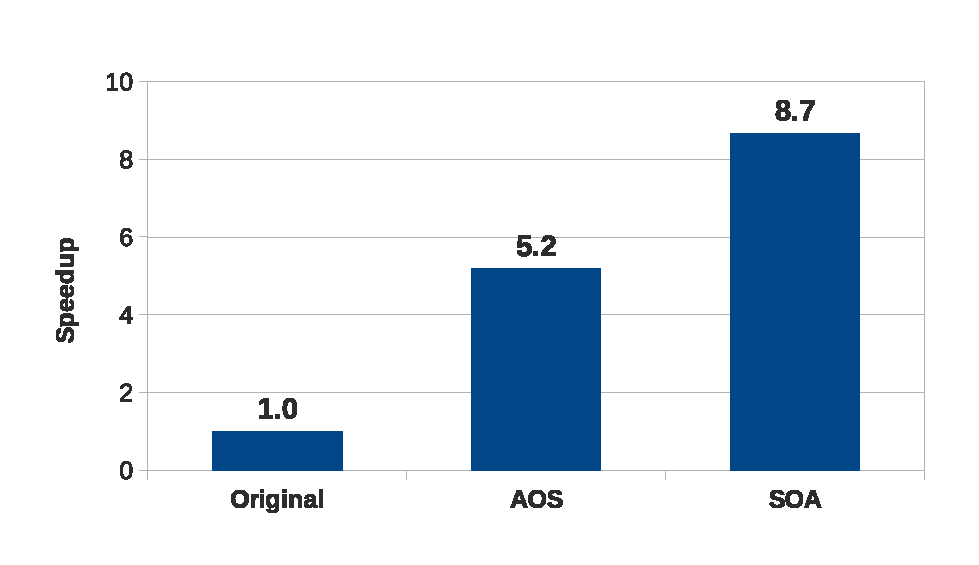
\includegraphics[width=\columnwidth]{images/graph_comparison_seq.eps}
	\caption{Speedup results for the three sequential versions, compared with the original version.}
	\label{fig:seq:results}
\end{figure}

\input{report/330-dependencies}
\section{Shared Memory}

A shared memory parallel version of \polu was implemented using the OpenMP interface. The main feature about this API is that the program itself remains almost equal to the sequential version, requiring only the addition of the necessary directives and the adaptation of the code to remove dependencies.

Both core functions were parallelized adding a \texttt{parallel for} directive to the internal loops. The number of threads issued in each parallel zone is given as the second argument of the program, and defaults to the maximum number of threads supported by the hardware in the absence of the argument.

\subsection{Load Balance}
\label{sec:omp:load}

\todorev{Last revised on Sat, June 30 at 22:18 by pfac}

Both core functions are mostly homogeneous in its parallel implementation.
In \computeflux, the two branches perform the same amount of operations whether they are followed or not.
In \update, the heaviest part of the workload is constant (products and divisions), and it only differs in the number of edges contributing to the cell.
While this value may cause the function to become heterogeneous, this is highly dependent on the mesh used (the test case used in this document has 3 edges in every cell).

By default, the OpenMP interface uses static scheduling, where iterations are assigned to threads in a \textit{round-robin} pattern.
Since the number of edges and cells is a constant throughout the entire execution, this guarantees the best load balancing among threads.

\subsection{Limitations}
% \todo[inline]{Describe the locality problems}
% \todo[inline]{Opportunity to show here that cute image that displays locality of the mesh}

The main problem with this implemetation is data locality. While these issues are softened using a SOA approach, and the method is a first order one, the algorithm is still not very cache friendly in either of the core functions.

In \computeflux, each edge requires access to data from the two adjacent cells. While the access to edges is contiguous, access to cells is not for most of the iterations. Yet, border edges do not require the second edge.

\update on the other hand requires access to all the edges in a cell, which are always more than two. Analogously, the access to cells is contiguous, but the access to edges is not. Since each edge has more edges, than an edge has adjacent cells, and since no edge may be neglect for any cell, this function is most likely the bottleneck of the main loop.
\section{Distributed Memory}
\label{sec:mpi}

\todorev{Last revised on Sat, June 30 at 23:25 at pfac}

For a distributed memory implementation, the \textit{Message Passing Interface} (MPI) was used.
With the sequential code having already suffered some changes and optimizations, the main problem consisted in the partitioning of the mesh.
The obvious approach is one where each processor is assigned to a subset of the entire mesh, and is responsible for the application of both kernels to its subset.
Communication is also required between each main loop iteration, since each process will require access to the values in the border of its subset, in order to compute its own values.

\subsection{Mesh Partitioning}
\label{subsec:mpi:partitioning}

\todorev{Last revised (with minor changes) on Sat, June 30 at 23:03 by pfac}

In order to distribute processing payload across each process, the input mesh, and all of the data associated with it, needs to be split into partitions.
A mesh partitioning algorithm is required. This algorithm must generate $P$ disjointed partitions (where $P$ is the number of processes), each to be assigned to a different process.
Some additional data is also required for each partition, so that information about how each partition connects to the others is kept, to allow communication to be done correctly.

\subsubsection{Research in Mesh Partitioning}
\label{subsubsec:mpi:partitioning:research}

Mesh partitioning is currently an actively researched topic, with some projects and libraries being already available to help understanding how a mesh (or more generically, a graph) can be partitioned in ways to optimize certain aspects like load balancing, communication balancing or partitioning overhead.
For instance, in \cite{metis}, a library called \texttt{Metis} is presented whose purpose is precisely this problem. Other works found for this topic include \cite{gilbert1995, walshaw2000}.

However, given the already mentioned time constraints of this project, and since the priority was to have a functional algorithm rather than an optimal one, it was decided not to attempt an approach involving \texttt{Metis} or any other researched work.
%Actually, the method used to partition the mesh is quite naive, as shown in \cref{subsubsec:mpi:partitioning:method}.

\subsubsection{Partitioning Methodology}
\label{subsubsec:mpi:partitioning:method}

The algorithm created to partition the mesh works by dividing it in slices by the horizontal coordinate of each cell.
Given a mesh with a total of $C$ cells, and a pool of $P$ processes, the mesh is divided into $P$ partitions, each with exactly $N=C/P$ cells, differing by at most one cell when they cannot be evenly divided.
By ordering the cells based on their horizontal coordinate, they are sequentially assigned to each process, in such a way that the first process receives the first $N$ cells of the set, and so on.

\begin{figure}[!htp]
	\begin{subfigure}[b]{0.5\columnwidth}
		\centering
		\includegraphics[width=\columnwidth]{foz_p2_msh}
		\caption{2 partitions}
		\label{fig:foz_p2_msh}
	\end{subfigure}%
	\begin{subfigure}[b]{0.5\columnwidth}
		\centering
		\includegraphics[width=\columnwidth]{foz_p4_msh}
		\caption{4 partitions}
		\label{fig:foz_p4_msh}
	\end{subfigure}%

	\caption{Mesh partitioning illustration}
	\label{fig:partitioning}
\end{figure}

With this partitioning method, communication is also greatly simplified, as it is guaranteed that every partition will have a left and a right neighbor.
It is also assumed that the width of the global mesh is big enough so that there are never processes with no cells assigned, which would break communication.
Since a common mesh usually contains at least thousands of cells, this should not be an issue.
The partitioning and assignment of the cells is done sequentially, thus it will increase preparation time.

\subsection{Communication Analysis}
\label{subsec:mpi:comm}

When computing the flux for a given edge, the pollution values of both adjacent cells are required. Until now, only one divergent case existed, when the edge was in the border of the mesh. With the addition of partitioning, a new divergence is created, when the edge is not in the border of the global mesh, but in the border of the local partition, meaning that one of its adjacent cells was assigned to a different partition.

A communication step is required at this point, so that each edge in the local border (the border that connects to another partition, not the global mesh border) receives the corresponding values from the neighbor partition 

This communication step was introduced at the beginning of the main loop, and consists of two smaller steps, one for left communication, and one for right communication.
Each iteration, every process starts by communicating the left border values, which were previously indexed in the preparation stage, to its left neighbor. Asynchronously with that task, it receives an equivalent message from the right neighbor, which is also at the same step. After both tasks, the direction of communication is reversed, and the right border values are sent to the right neighbor of each partition.

Only after all communication is done for this process can it continue to the main kernels of the loop. This introduces a large overhead, as it will most likely require a network transfer if the neighbor partition is located in a different machine. This overhead may become a huge bottleneck for the loop, especially for smaller inputs, where the time spent in the kernels is small enough to make the partitioning and communication occupy a large percentage of the program.

An alternative could consist in making the communication an asynchronous task, allowing the flux for inner edges to be computed while the communication is taking place, since they don't depend on the values to be received. Again, due to time constraints, it was not possible to better analyse this solution.

\subsection{Load Balance}
\label{subsec:mpi:load}

\todo[inline,color=green!40]{Describe how the mesh was partitioned}

With the naive partitioning strategy used, load balance becomes a problem. The computation itself is actually well balanced, since it is assured that every partition has the same amount of cells (differing at most by one). The problem is in the border between those partitions. With the division by the $x$ coordinate being used, it becomes obvious that the size of the border between partitions becomes extremely dependant on the format of the mesh itself. Other approaches, already mentioned in \cref{subsubsec:mpi:partitioning:research} attempt to deal with this, and produce partitions that minimize the size of the border.

The drawback of not controlling border sizes comes at the communcation step. Not only could there be different partitioning solutions that could minimize the border, thus minimizing the amount of data transfered, it can also happen that different partitions have very different border sizes, compromising communication balance.

\subsection{Results}
\label{sec:mpi:results}

These results show the attained speedups for the MPI implementation. Due to SeARCH limitations, only tests with two nodes were able to run (see \cref{sec:env, sec:method} for further details). Speedups are compared against the original sequencial version in \cref{fig:mpi:results}.

\begin{figure}[!htp]
	\centering
	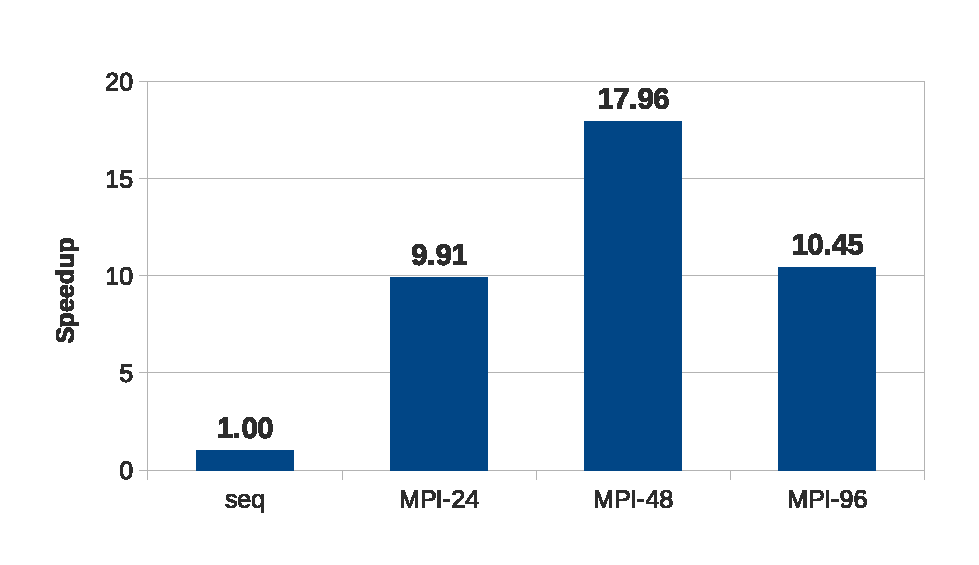
\includegraphics[width=\columnwidth]{graph_comparison_mpi}
	\caption{MPI implementation speedups}
	\label{fig:cuda:results}
\end{figure}

While there are actual speedups, especially for 48 processes, the results are not as good as the OpenMP results. The reason for this comes from the nature of the algorithm, that makes it very sensible to the overhead of communications. This imposes large limits to the scalability of any shared memory implementation of \polu.


\section{CUDA Implementation}
\label{sec:600}

\todosec{CUDA implementation}
Part of the work of this project was to study the parallelization methods and issues of the studied schemes in a massively parallel architecture, specifically a GPU, using CUDA as the development technology. Some considerations can be made about the parallelization of each of the schemes presented.

The first-order scheme is clearly the one where the translation to a massively parallel implementation is straightforward. Each value of the solution at the end of each iteration is being computed based solely on the strictly adjacent elements of the mesh. The higher locality gained from only using adjacent values for each edge allows for much greater locality and less memory overhead than the second-order counterparts.

As for the second-order schemes, such a straightforward solution is not possible, or at least not with the same ratio of performance gain when compared to a first-order scheme. This is due to the more irregular nature of these schemes.
In the reconstruction phase, we need access to the immediate neighbours of each cell. In a two dimensional mesh, the number of neighbours is arbitrary, and it is not possible to perfectly serialize each cell in memory. This results in a higher memory access cost, since we can't take as much advantage of the GPU's coalesced memory accesses at this step.

As for the two second-order approaches tested, while the {\it a posteriori} solution with the MOOD method provides a better numerical result, it also comes with a performance cost, when compared to the MUSCL method. This is mostly due to the recalculations that are necessary in the inner computations of the correct flux, which is iteratively updated until there are no more problematic values. This introduces a bottleneck, particularly noticeable in a parallel environment, since every successive iteration will only deal with a smaller amount of data than the previous one, as the amount of invalid values is reduced.
In the MUSCL method we also have a higher amount of divergence than the first-order scheme. This is not as significant as in the MOOD method, however.
Both of these conclusions seem to suggest that the {\it a priori} approach allows for a better, more regular parallelization in a massively parallel architecture.

Some more elaborate optimizations have been proposed for the second-order schemes, which might help achieve performances near the first-order scheme. One possible optimization would be to partition the mesh, allowing different chunks to be processed independently. This would allow chunks that have already been completely processed to advance further in time without waiting for the global iteration to finish, and would possibly help hide the latency from the MOOD method value correction. Since the amount of values to fix is usually small, having different partitions in different states would allow for partitions that had already been completely corrected to continue on, and effectively increase the usage of the device.
Another possibility would be the addition of coherence control, by controling the serialization of the mesh, and the cells being processed at each time. The application does not perform any preprocessing on the mesh organization, thus relying on the mesh generator to generate a compute-friendly input data. This might result in a mesh layout that does not take into account the advantages that can be gained in terms of performance by exploiting locality. A strategy that would reorder the mesh by maximizing the correlation between the physical element distance and their distance in the memory space would increase locality and consequentely, performance on all employed methods, including the first-order scheme.

\section{Final results}
\subsection{Results}
\todo[inline]{Only describe the results, a.k.a. translate every chart to words}
\subsection{Analysis}
\todo[inline]{Interpret every chart. Say what each means, what can be concluded from it}
\todo[inline]{Merge this subsection with the results if time is of the essence}
\section{Conclusion}
\label{sec:conclusion}

\todo[inline]{Sum all this shit up.}
\todo[inline,color=green!40]{Or in my own words: Sum the fuck out of this shit}
\todopfac{Mencionar localidade como trabalho futuro.}
\todo[inline]{Referir que apesar dos speedups de CUDA não serem tão melhores que os outros como se esperava, isso pode dever-se ao facto de que não nos foi possivel gerar um input grande o suficiente para tirar o maximo partido do hardware do GPU}


%
% BIBLIOGRAPHY
%
\bibliographystyle{IEEEtran}
\bibliography{../bib/strings,../bib/articles,../bib/inproceedings,../bib/manuals,../bib/misc,../bib/techreports}

% \printbibliography

%
% APPENDIXES
%

\appendices
\section{Environmental Setup}
\label{sec:env}

\todo[inline]{Describe the hex nodes}
\todo[inline]{Add a roofline for each type of nodes described}
\todo[inline]{Calculate Amdahl's Law for each hardware group}

\section{Experiment Methodology}
\label[appendix]{sec:method}

\todo[inline]{Explain the hows and whys of the latest methodology}
\todo[inline]{Add the methodologies from all the phases which were not retested}
\todo[inline]{No problem in sending this to an appendix -> and it should}

\section{Roofline}
\label[appendix]{sec:roofline}

The roofline model used in this document was prepared according to the guidelines in \cite{williams08}, except for the memory bandwidth roof and some adaptations. Compared to operational intensity, computational intensity (or arithmetic intensity) is a more complete measure for the program studied in this document.

As stated in \cref{sec:env}, the roofline model presented in this document refers to a very specific node of SeARCH Group 201.

According to \cite{xeon5100,intelsys,inteloptimize}, these nodes' micro architecture is \intel Core\texttrademark, which is capable of decoding up to five instructions per cycle, has a throughput of up to 4 instructions per cycle and three full arithmetic logical units, where each has a throughput of one instruction per cycle for many kinds of computational instructions. This binds the peak throughput of computational instructions at 3 per cycle.

Since each core has a peak throughput of 3 computational instructions per cycle, each processor has 2 cores at a clock frequency of 2.0 GHz, and each node has 2 processors, this results in a peak of
\begin{IEEEeqnarray}{rCl}
3\times 2\times 2\times 10^{9}\times 2 & = & 24\;\mathrm{GInstructions/s}\enspace .
\end{IEEEeqnarray}
This value corresponds to the CPU roof.

Although \cite{williams08} recommends using ``a series of highly tuned versions of the STREAM benchmark'', the creation of such versions is out of the scope of this project. As such, the peak memory bandwidth was measured running the original STREAM benchmark in a SeARCH Group 201 node. The benchmark returned a peak value of 4.78 GB/s, which is the memory roof.

As for CPU ceilings, these were calculated decreasing the number of cores used, first by using only one processor (half the peak), then by removing thread-level parallelism (one core, a quarter of the peak). As measured in the previous report, this algorithm already presents itself with a high balance of floating-point multiplications and additions (two thirds of the TLP ceiling, as one of the ALUs would remain idle). The last CPU ceiling remaining would mean removing all the instruction-level parallelism (half the Mul/Add balance ceiling, only one ALU active).

Lastly, the absence of dual channel was used as the only memory ceiling. The influence of any other mechanism such as prefetch or unit stride accesses would have to be properly measured with the recommended tuned versions, which are not available for this document.

\Cref{fig:roofline} shows the resulting roofline model for the nodes of SeARCH Group 201.

\begin{figure}[!htp]
	\begin{center}
		\includegraphics[width=\columnwidth]{images/roofline201}
	\end{center}
	\caption{Roofline for SeARCH Group 201.}
	\label{fig:roofline}
\end{figure}




\end{document}
